\documentclass{standalone}

% User packages:
% ======================================================================
\usepackage{amsmath}
\usepackage{amsfonts}
\usepackage{amssymb}
\usepackage{graphicx}
\usepackage{epsfig}
\usepackage[hang,nooneline]{subfigure}
\usepackage[normalem]{ulem}
\usepackage{color}
\usepackage{braket}
\usepackage{hyperref}
\usepackage{todonotes}
\usepackage{algorithm}
\usepackage{multirow}
\usepackage{hhline}
\usepackage{shortvrb}
\usepackage{cprotect}
\usepackage[noend]{algpseudocode}
\usepackage{overpic}
\usepackage{cleveref}

% Tikz plot
\usepackage{csvsimple}
\usepackage{tikz}
\usepackage{pgfplots}
\usepgfplotslibrary{colorbrewer}

\makeatletter

\def\pgfplots@getautoplotspec into#1{%
    \begingroup
    \let#1=\pgfutil@empty
    \pgfkeysgetvalue{/pgfplots/cycle multi list/@dim}\pgfplots@cycle@dim
    %
    \let\pgfplots@listindex=\pgfplots@numplots
    %%% Start new code
    \pgfkeysgetvalue{/pgfplots/cycle list set}\pgfplots@listindex@set
    \ifx\pgfplots@listindex@set\pgfutil@empty
    \else 
        \c@pgf@counta=\pgfplots@listindex
        \c@pgf@countb=\pgfplots@listindex@set
        \advance\c@pgf@countb by -\c@pgf@counta
        \globaldefs=1\relax
        \edef\setshift{%
            \noexpand\pgfkeys{
                /pgfplots/cycle list shift=\the\c@pgf@countb,
                /pgfplots/cycle list set=
            }
        }%
        \setshift%
    \fi
    %%% End new code    
    \pgfkeysgetvalue{/pgfplots/cycle list shift}\pgfplots@listindex@shift
    \ifx\pgfplots@listindex@shift\pgfutil@empty
    \else
        \c@pgf@counta=\pgfplots@listindex\relax
        \advance\c@pgf@counta by\pgfplots@listindex@shift\relax
        \ifnum\c@pgf@counta<0
            \c@pgf@counta=-\c@pgf@counta
        \fi
        \edef\pgfplots@listindex{\the\c@pgf@counta}%
    \fi
    \ifnum\pgfplots@cycle@dim>0
        % use the 'cycle multi list' feature.
        %
        % it employs a scalar -> multiindex map like
        % void fromScalar( size_t d, size_t scalar, size_t* Iout, const size_t* N )
        % {
        %   size_t ret=scalar;
        %   for( int i = d-1; i>=0; --i ) {
        %       Iout[i] = ret % N[i];
        %       ret /= N[i];
        %   }
        % }
        % to get the different indices into the cycle lists.
        %-------------------------------------------------- 
        \c@pgf@counta=\pgfplots@cycle@dim\relax
        \c@pgf@countb=\pgfplots@listindex\relax
        \advance\c@pgf@counta by-1
        \pgfplotsloop{%
            \ifnum\c@pgf@counta<0
                \pgfplotsloopcontinuefalse
            \else
                \pgfplotsloopcontinuetrue
            \fi
        }{%
            \pgfkeysgetvalue{/pgfplots/cycle multi list/@N\the\c@pgf@counta}\pgfplots@cycle@N
            % compute list index:
            \pgfplotsmathmodint{\c@pgf@countb}{\pgfplots@cycle@N}%
            \divide\c@pgf@countb by \pgfplots@cycle@N\relax
            %
            \expandafter\pgfplots@getautoplotspec@
                \csname pgfp@cyclist@/pgfplots/cycle multi list/@list\the\c@pgf@counta @\endcsname
                {\pgfplots@cycle@N}%
                {\pgfmathresult}%
            \t@pgfplots@toka=\expandafter{#1,}%
            \t@pgfplots@tokb=\expandafter{\pgfplotsretval}%
            \edef#1{\the\t@pgfplots@toka\the\t@pgfplots@tokb}%
            \advance\c@pgf@counta by-1
        }%
    \else
        % normal cycle list:
        \pgfplotslistsize\autoplotspeclist\to\c@pgf@countd
        \pgfplots@getautoplotspec@{\autoplotspeclist}{\c@pgf@countd}{\pgfplots@listindex}%
        \let#1=\pgfplotsretval
    \fi
    \pgfmath@smuggleone#1%
    \endgroup
}

\pgfplotsset{
    cycle list set/.initial=
}
\pgfplotsset{cycle list/Set1}

\colorlet{MyGreen}{green!50!black}

\usetikzlibrary{external}
% Comment out the next three lines for faster compilation time
\usepgfplotslibrary{external}
\pgfplotsset{compat=1.15}
\tikzexternalize[optimize=false,prefix=fig/] % or false


%%% MIKTEX options
\tikzset{external/system call= {lualatex
                           -enable-write18
                           -halt-on-error 
                           -shell-escape 
                           -synctex=1
                           -interaction=nonstopmode
                           -jobname "\image" "\texsource"}}
\begin{document}
\tikzset{>=latex}

%%
\def\branchid{}
\tikzsetnextfilename{figure_branch_\branchid}
\begin{tikzpicture}
\begin{axis}[xmin=2.0*10^4, xmax=10^5, enlargelimits=false, x label style={at={(0.5,-0.07)}}, xlabel={$\textrm{Ra}$},y label style={at={(-0.2,0.4)},rotate=-90,anchor=south},ylabel={$\|\mathbf{u}\|_2^2$}, every x tick scale label/.style={at={(xticklabel cs:1)},anchor=south west, yshift=-0.11em},xtick scale label code/.code={\pgfmathparse{int(#1)}$\times 10^{\pgfmathresult}$}]
\addplot[blue,line width=0.6] table [col sep=comma, smooth,mark=none] {data/diagram_u/\branchid.csv};

\node at (axis cs:3.3*10^4,400) (A1) {};
\node at (axis cs:23400,4.80e-1) (B1) {};
\draw [->] (A1.center) -- (B1.center);
\node[inner sep=0pt] (test) at (axis cs:3.3*10^4,400)
    {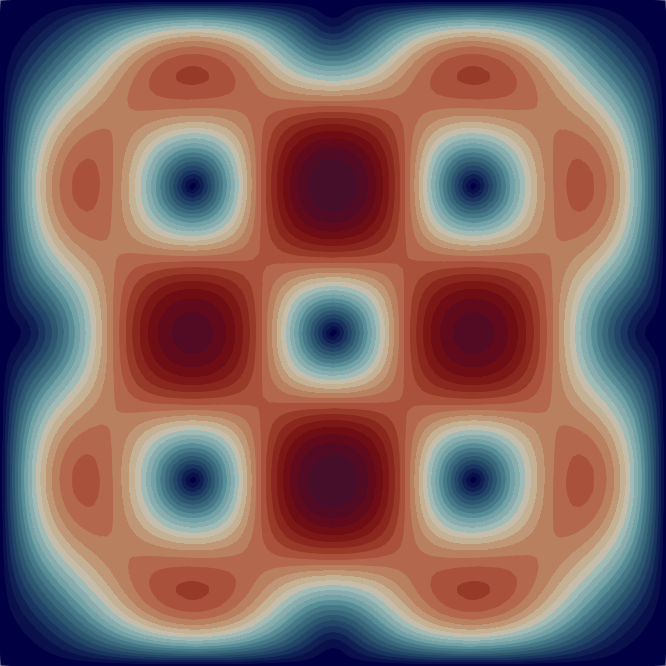
\includegraphics[width=.1\textwidth]{data/Figure_paper/34/u_23400.png}};

\node at (axis cs:5.5*10^4,900) (A1) {};
\node at (axis cs:63850,5.685325552611886906e+02) (B1) {};
\draw [->] (A1.center) -- (B1.center);
\node[inner sep=0pt] (test) at (axis cs:5.5*10^4,900)
    {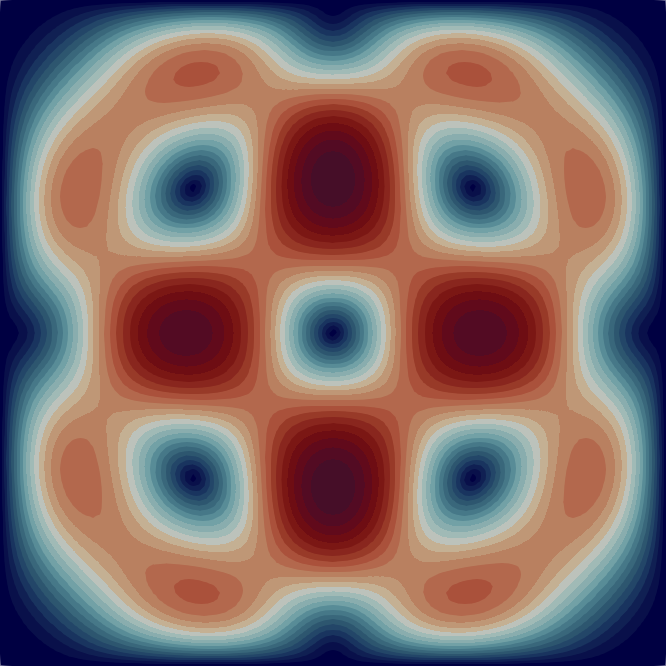
\includegraphics[width=.1\textwidth]{data/Figure_paper/34/u_63850.png}};

\node at (axis cs:9*10^4,700) (A1) {};
\node at (axis cs:10^5,1.176752550618319447e+03) (B1) {};
\draw [->] (A1.center) -- (B1.center);
\node[inner sep=0pt] (test) at (axis cs:9*10^4,700)
    {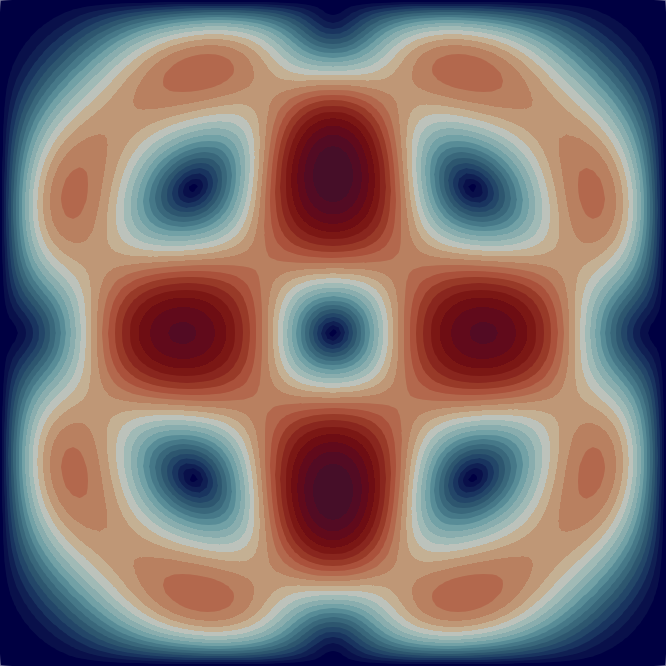
\includegraphics[width=.1\textwidth]{data/Figure_paper/34/u_100000.png}};
\end{axis}

\begin{axis}[yshift=-105mm, yscale=0.45, xmin=2*10^4, xmax=10^5, ymin=-50, ytick distance=50, enlargelimits=false, x label style={at={(0.5,-0.3)}}, xlabel={$\textrm{Ra}$},y label style={at={(-0.2,0.8)},rotate=-90,anchor=south},ylabel={$\mathcal{R}(\lambda)$}, every x tick scale label/.style={at={(xticklabel cs:1)},anchor=south west, yshift=-0.86em},xtick scale label code/.code={\pgfmathparse{int(#1)}$\times 10^{\pgfmathresult}$}, ]

\pgfplotsset{cycle list set=1}
\foreach \i in {2,3,4,5,6}{
\addplot+[only marks, mark size=0.4] table [col sep=comma] {data/StabilityFigures/\branchid_real_\i.csv};
}
\pgfplotsset{cycle list set=6}
\addplot+[only marks, mark size=0.4] table [col sep=comma] {data/StabilityFigures/\branchid_real_8.csv};

\pgfplotsset{cycle list set=0}
\addplot+[only marks, mark size=0.4] table [col sep=comma] {data/StabilityFigures/\branchid_real_1.csv};

\draw[black,line width=0.6] 
  (axis cs:\pgfkeysvalueof{/pgfplots/xmin},0) -- 
  (axis cs:\pgfkeysvalueof{/pgfplots/xmax},0);
\end{axis}

%%
\begin{axis}[xshift=95mm, xmin=2*10^4, xmax=10^5, enlargelimits=false, x label style={at={(0.5,-0.07)}}, xlabel={$\textrm{Ra}$},y label style={at={(-0.2,0.4)},rotate=-90,anchor=south},ylabel={$\|T\|_2^2$}, every x tick scale label/.style={at={(xticklabel cs:1)},anchor=south west, yshift=-0.11em},xtick scale label code/.code={\pgfmathparse{int(#1)}$\times 10^{\pgfmathresult}$}]
\addplot[blue,line width=0.6] table [col sep=comma, smooth,mark=none] {data/diagram_T/\branchid.csv};
    
\node at (axis cs:3*10^4,0.315) (A1) {};
\node at (axis cs:23400,3.333033177180729223e-01) (B1) {};
\draw [->] (A1.center) -- (B1.center);
\node[inner sep=0pt] (test) at (axis cs:3*10^4,0.315)
    {
\includegraphics[width=.1\textwidth]{data/Figure_paper/34/T_23400.png}};

\node at (axis cs:5.5*10^4,0.327) (A1) {};
\node at (axis cs:63850,3.147133966794487536e-01) (B1) {};
\draw [->] (A1.center) -- (B1.center);
\node[inner sep=0pt] (test) at (axis cs:5.5*10^4,0.327)
    {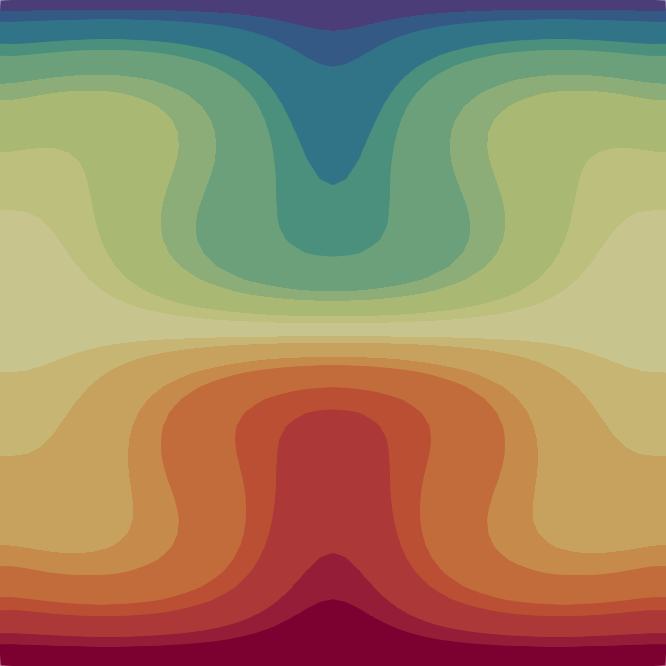
\includegraphics[width=.1\textwidth]{data/Figure_paper/34/T_63850.png}};

\node at (axis cs:8.5*10^4,0.32) (A1) {};
\node at (axis cs:10^5,3.090847496538097761e-01) (B1) {};
\draw [->] (A1.center) -- (B1.center);
\node[inner sep=0pt] (test) at (axis cs:8.5*10^4,0.32)
    {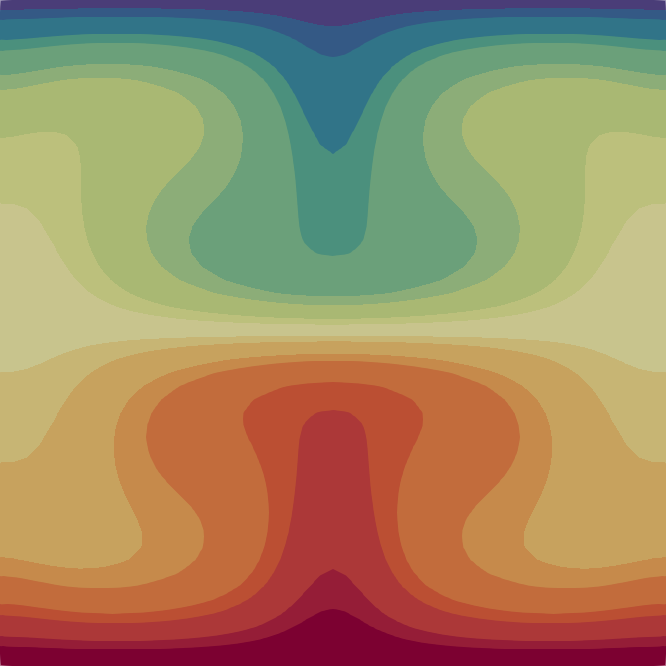
\includegraphics[width=.1\textwidth]{data/Figure_paper/34/T_100000.png}};
    
\end{axis}

\begin{axis}[xshift=95mm, yshift=-105mm, yscale=0.45, xmin=2*10^4, xmax=10^5, ymin=0, ymax=150, enlargelimits=false, x label style={at={(0.5,-0.3)}}, xlabel={$\textrm{Ra}$},y label style={at={(-0.2,0.8)},rotate=-90,anchor=south},ylabel={$\mathcal{I}(\lambda)$}, every x tick scale label/.style={at={(xticklabel cs:1)},anchor=south west, yshift=-0.86em},xtick scale label code/.code={\pgfmathparse{int(#1)}$\times 10^{\pgfmathresult}$}, ]

\pgfplotsset{cycle list set=1}
\foreach \i in {2,3,4,5,6}{
\addplot+[only marks, mark size=0.4] table [col sep=comma] {data/StabilityFigures/\branchid_imag_\i.csv};
}

\pgfplotsset{cycle list set=0}
\addplot+[only marks, mark size=0.4] table [col sep=comma] {data/StabilityFigures/\branchid_imag_1.csv};

\end{axis}

\begin{axis}[xshift=50mm, yshift=-70mm, xmin=2*10^4, xmax=10^5, enlargelimits=false, x label style={at={(0.5,-0.07)}}, xlabel={$\textrm{Ra}$},y label style={at={(-0.2,0.4)},rotate=-90,anchor=south},ylabel={$\|\mathbf{B}\|_2^2$}, every x tick scale label/.style={at={(xticklabel cs:1)},anchor=south west, yshift=-0.11em},xtick scale label code/.code={\pgfmathparse{int(#1)}$\times 10^{\pgfmathresult}$}]
\addplot[blue,line width=0.6] table [col sep=comma, smooth,mark=none] {data/diagram_B/\branchid.csv};
    
\node at (axis cs:3*10^4,0.315) (A1) {};
\node at (axis cs:23400,3.333033177180729223e-01) (B1) {};
\draw [->] (A1.center) -- (B1.center);
\node[inner sep=0pt] (test) at (axis cs:3*10^4,0.315)
    {
\includegraphics[width=.1\textwidth]{data/Figure_paper/34/T_23400.png}};

\node at (axis cs:5.5*10^4,0.327) (A1) {};
\node at (axis cs:63850,3.147133966794487536e-01) (B1) {};
\draw [->] (A1.center) -- (B1.center);
\node[inner sep=0pt] (test) at (axis cs:5.5*10^4,0.327)
    {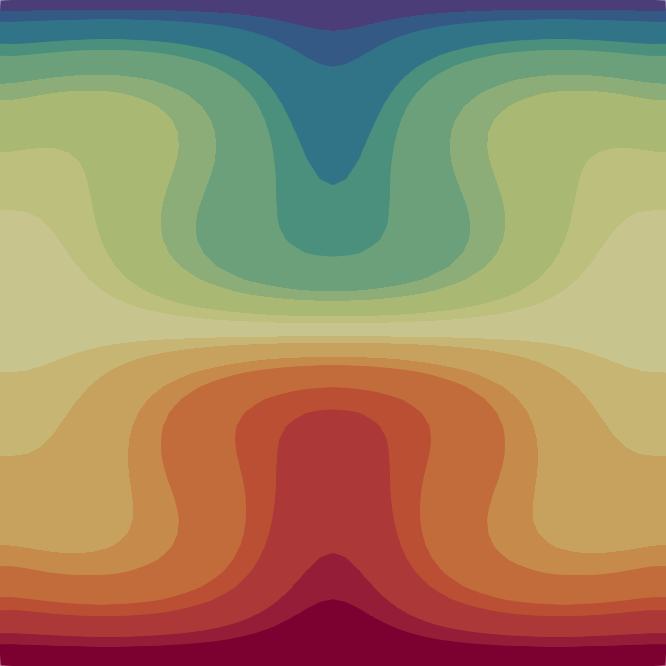
\includegraphics[width=.1\textwidth]{data/Figure_paper/34/T_63850.png}};

\node at (axis cs:8.5*10^4,0.32) (A1) {};
\node at (axis cs:10^5,3.090847496538097761e-01) (B1) {};
\draw [->] (A1.center) -- (B1.center);
\node[inner sep=0pt] (test) at (axis cs:8.5*10^4,0.32)
    {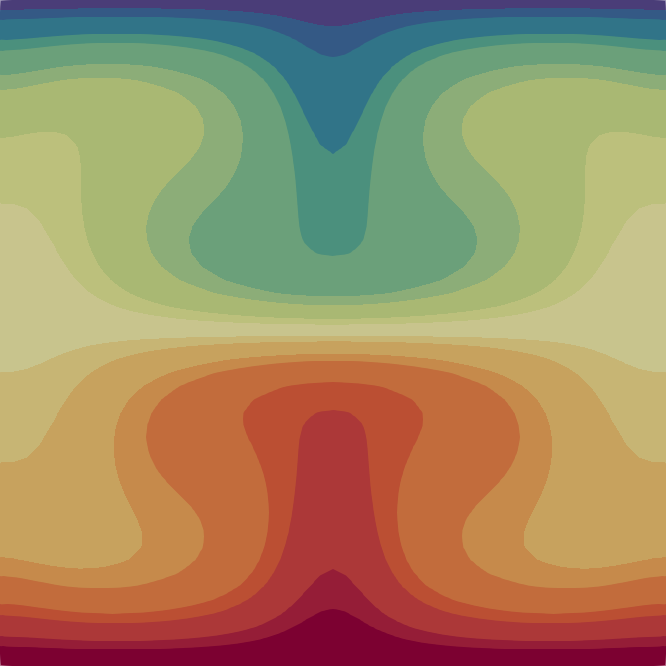
\includegraphics[width=.1\textwidth]{data/Figure_paper/34/T_100000.png}};
    
\end{axis}

\end{tikzpicture}

\end{document}
